We used randomly generated non-private IP addresses and movie titles with \texttt{.avi} endings as keys for nodes and extents respectively. This was done to make the experiment more applicable to real scenarios. Java's standard library was used for SHA-1 hashing. A consistent hashing algorithm, to balance the load of nodes. Our identifier circle was $[0,2^{40})$ which was large enough to avoid collisions.

We initialized the DHT with $10$ nodes and $10^4$ extents. In each iteration we picked a random node and made it request $10^6$ writes to random extents. We then added $5$ more nodes to the DHT and performed the writes again until a node count of $30$ was reached. The parameters used are summarized in Table \ref{tab:params}.
\begin{table}[ht!]
    \centering
    \scalebox{0.9}{
    \begin{tabular}{c|l|c}
        $S$ & Number of nodes initially & $10$\\
        \hline
        $E$ & Number of extents & $10^4$\\
        \hline
        $N$ & Copies of each extent & $3$\\
        \hline
        $W$ & Writes each iteration & $10^6$\\
        \hline
        $I$ & Nodes added in each iteration & $5$\\
        \hline
        $S_m$ & Maximum number of nodes & $30$\\ 
    \end{tabular}
    }
    \caption{The parameters used for our experiment.}
    \label{tab:params}
\end{table}
Every write was tracked, both for nodes and extents. After each iteration we reset the write counters so we could compare if the distribution of writes for nodes was analogous to the distribution of extents assigned to nodes. That way we avoid biasing older nodes. The distributions for 10 and 30 nodes can be seen in Figure \ref{fig:dist10} and Figure \ref{fig:dist30} respectively. The standard deviation of these distributions for all number of nodes can be seen in Table \ref{tab:stddev}.

\begin{figure}[ht!]
    \centering
    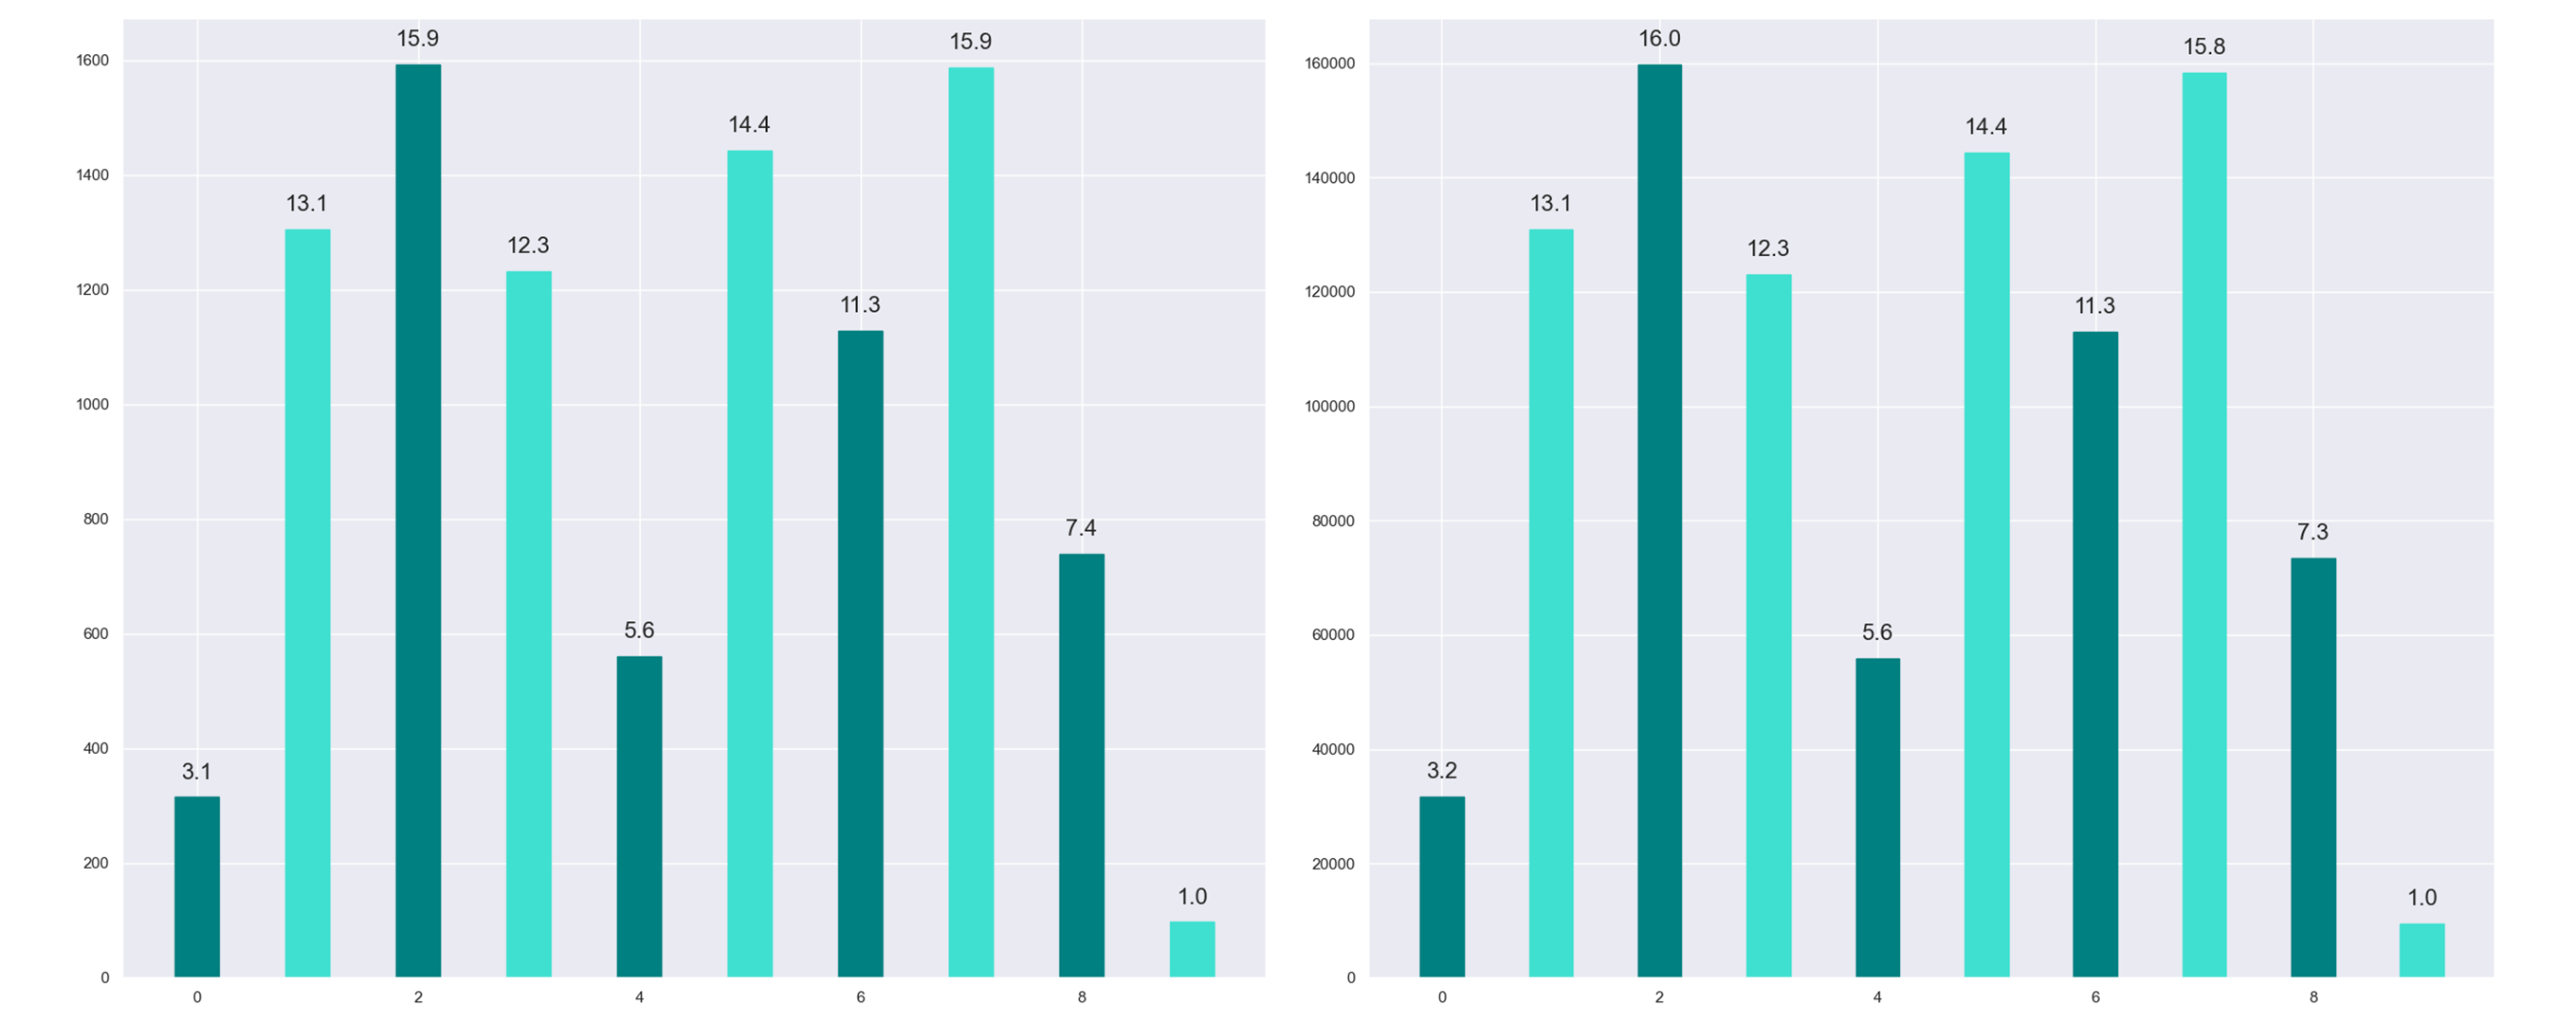
\includegraphics[scale=.075]{img/dist10nodes.png}
    \caption{The distribution of extents over 10 nodes on the left and distribution of writes over the same nodes on the right.}
    \label{fig:dist10}
\end{figure}
\begin{figure}[ht!]
    \centering
    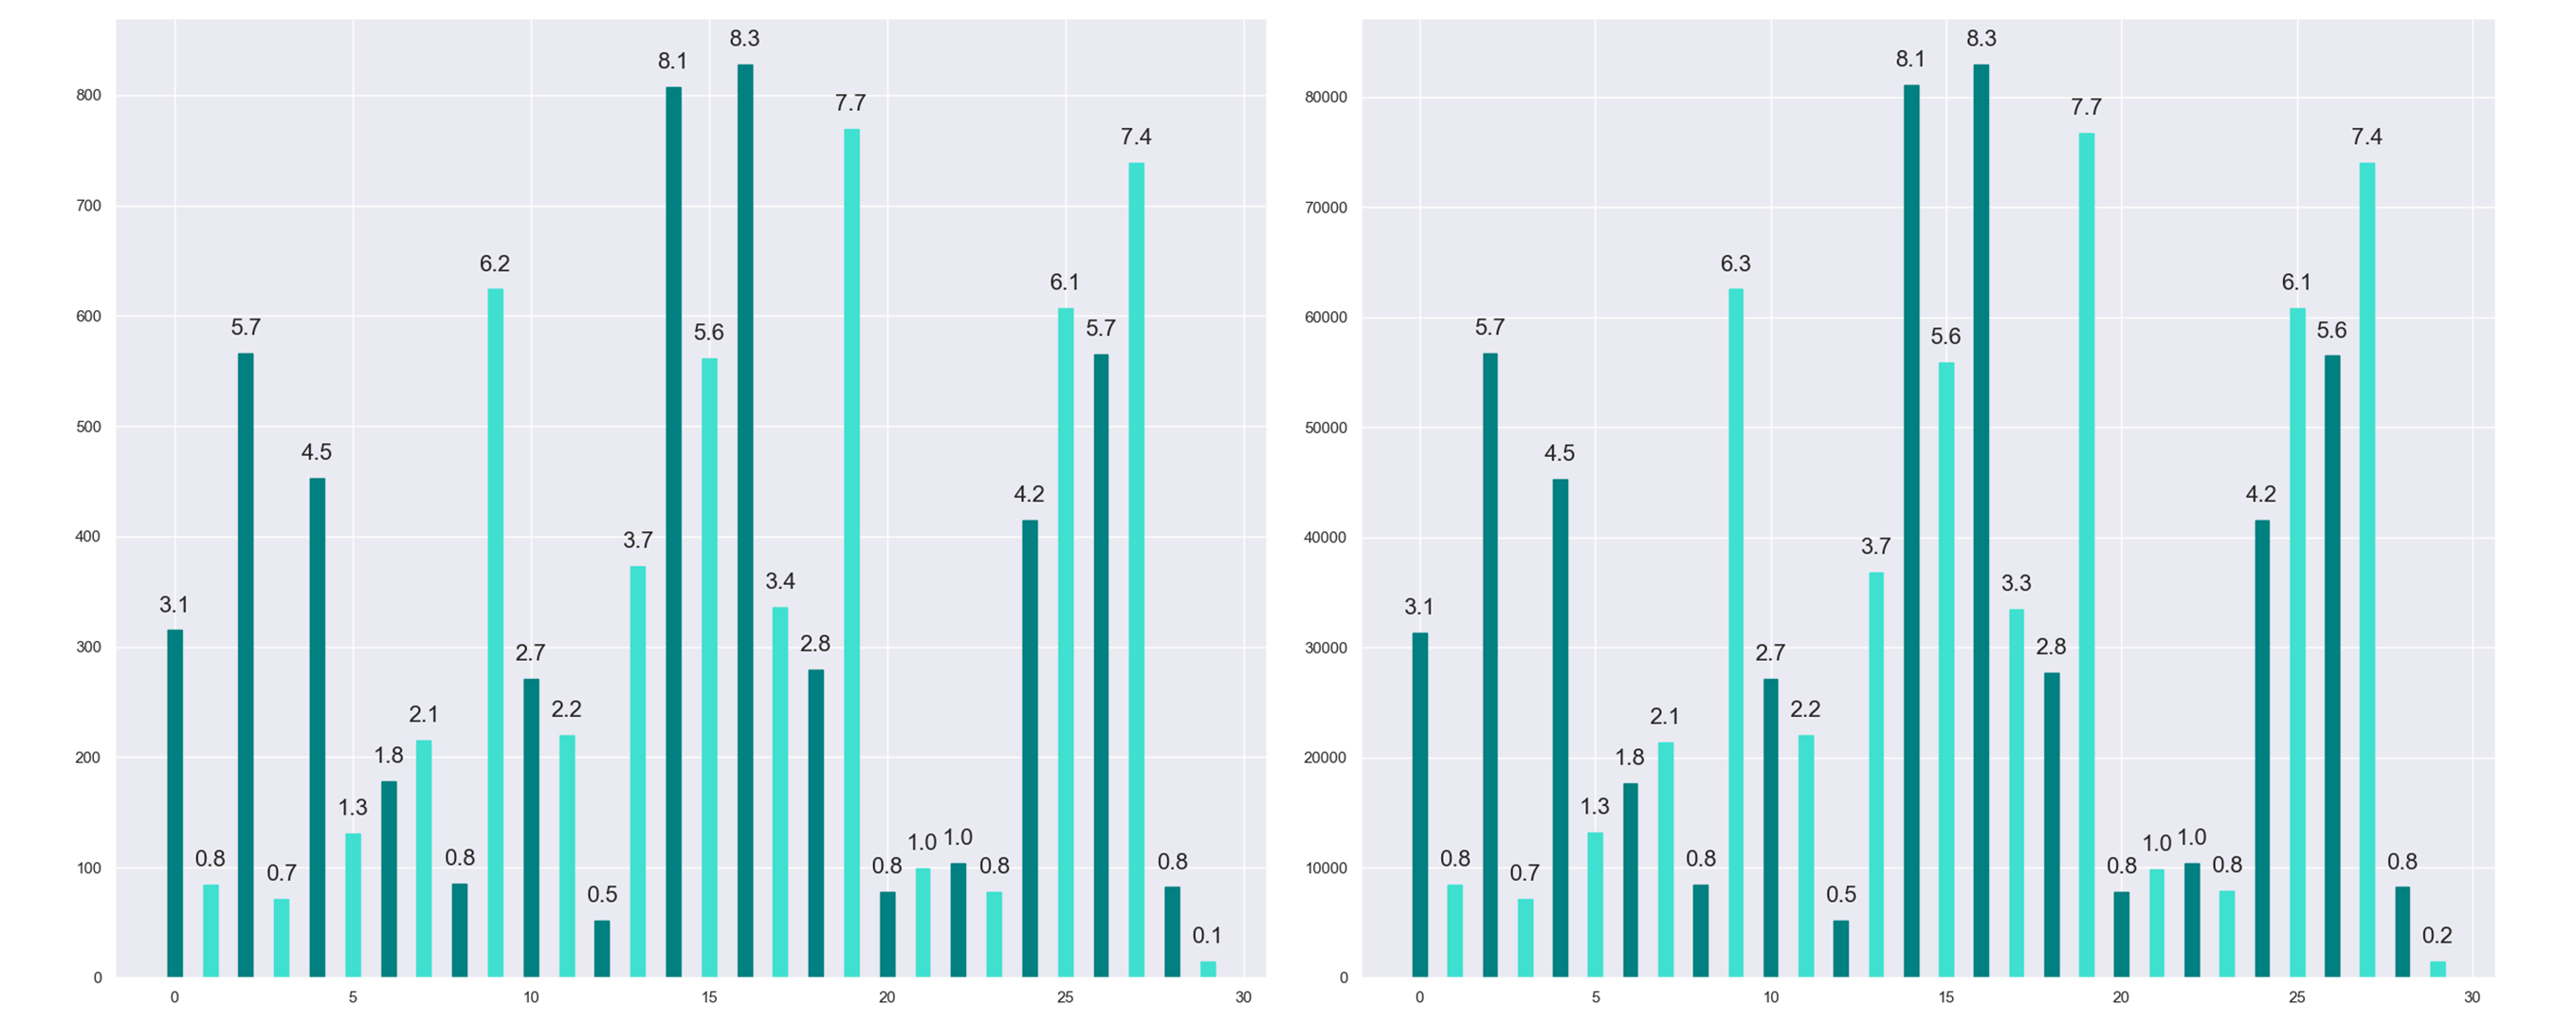
\includegraphics[scale=.075]{img/dist30nodes.png}
    \caption{The distribution of extents over 30 nodes (20 added to the original 10) on the left and distribution of writes over the same nodes on the right.}
    \label{fig:dist30}
\end{figure}

\begin{table}[ht!]
    \centering
    \scalebox{0.65}{
    \begin{tabular}{c|ccccc}
        $S$ & 10 & 15 & 20 & 25 & 30\\
        \hline
        $\mu_{\text{extents}}$ & 537.61 & 382.75 & 353.02 & 314.04 & 258.53\\
        \hline
        $\sigma_\text{writes}$ &53848.17 & 38224.04 & 35254.81 & 31456.25 & 25866.75
    \end{tabular}
    %\begin{tabular}{c|c|c}
    %    $S$ & $\mu_{\text{extents}}$ & $\sigma_\text{writes}$ \\
    %    \hline
    %    10 & 537.61 & 53848.17\\
    %    15 & 382.75 & 38224.04\\
    %    20 & 353.02 & 35254.81\\
    %    25 & 314.04 & 31456.25\\
    %    30 & 258.53 & 25866.75
    %\end{tabular}
    }
    \caption{Standard deviation of extents and writes over nodes.}
    \label{tab:stddev}
\end{table}

We also tracked jumps when finding successor nodes but only did so with writes. Their distribution can be seen in Figure \ref{fig:jumps} for 10 and 30 nodes. 
\begin{figure}[ht!]
    \centering
    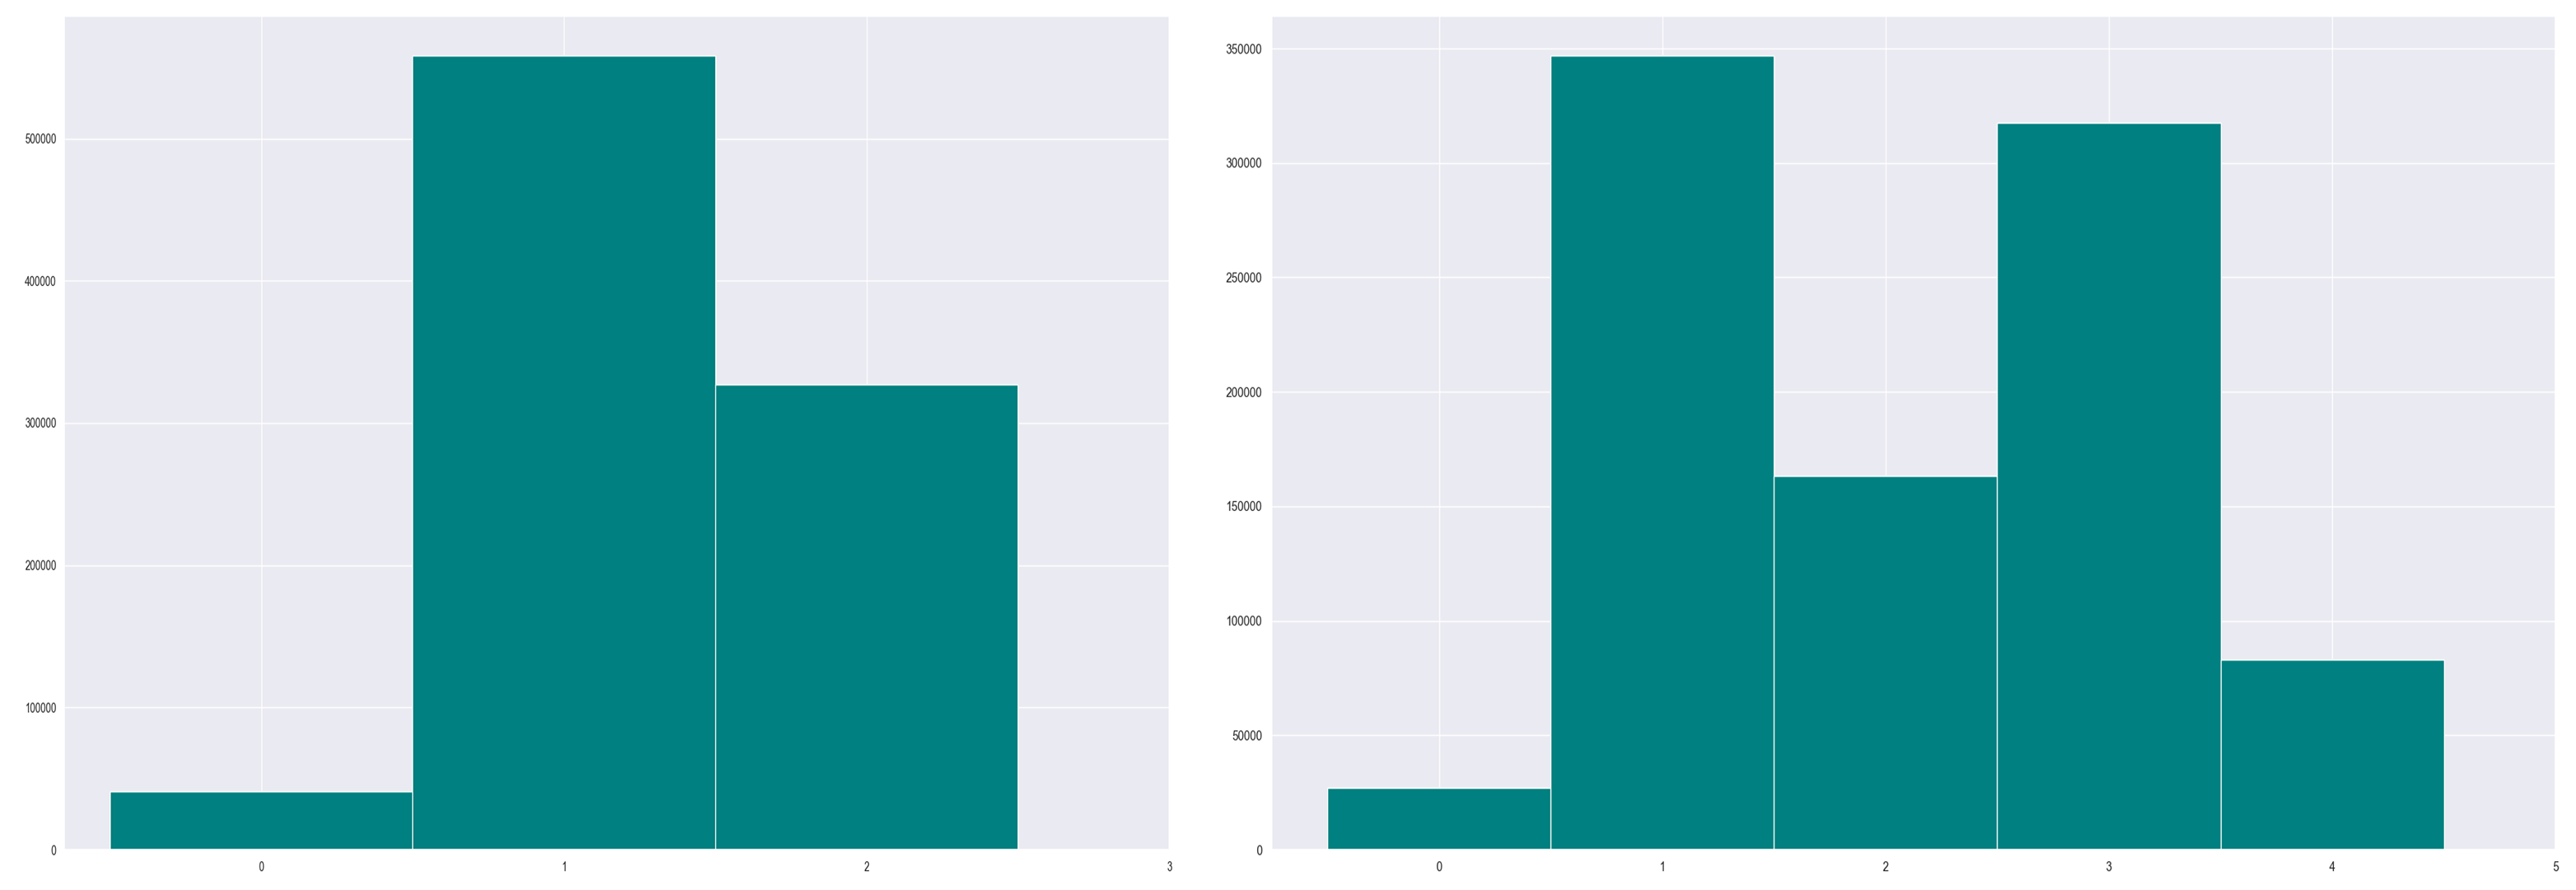
\includegraphics[scale=0.065]{img/jumps.png}
    \caption{The distribution of number of jumps for 10 (left) and 30 (right) nodes.}
    \label{fig:jumps}
\end{figure}